\subsection{Сравнительный анализ схем приводов газоперекачивающих агрегатов}

\subsubsection{Обзор существующих схем}
Одной из особенностей эксплуатации газотурбинных установок (ГТУ) в качестве привода ГПА является практически постоянная
работа установки на режимах частичной мощности ~\cite{gtd_oil_and_gas}. В связи с этим на этапе вариантного проектирования
привода ГПА необходимо проводить сравнительную оценку рассматриваемых вариантов в широком диапазоне рабочих мощностей.

В данной работе проводится анализ эффективности работы газотурбинных двигателей различных схем в диапазоне мощностей
30-100\% номинальной мощности и дается оценка эффективности использования ГТУ таких схем в качестве приводов ГПА.

Газотурбинные установки ГПА могут быть разделены на изначально стационарные и конвертированные из авиационных и судовых двигателей.

Все стационарные установки, за исключением ГТ-700-4 и ГТК-25, двухвальные (ГТ-700-4 – одновальная, ГТК-25 - трехвальная).
Камеры сгорания стационарных ГТУ индивидуальные, находятся вне корпусов турбин и представляют собой либо одну камеру
цилиндрической формы, установленную вертикально или горизонтально, либо несколько секционных камер малого объема,
равномерно расположенных по периметру ТВД (ГТН-16 и ГТН-25) ~\cite{gtd_tomsk}.

Газотурбинные установки на базе авиационных двигателей являются продуктом конвертирования авиационных турбин. Перед
установкой авиационных двигателей на ГПА они переводятся с жидкого топлива на газовое.

Для транспорта используются главным образом двигатели авиалайнеров Ту 114 и Ту 154, НК-12МВ и НК-8-2У с маркировкой
после конвертации НК-12СТ и НК-16СТ – мощностью соответственно 6,3 МВт и 16 МВт. Первый из приведенных двигателей входит
в состав газоперекачивающего агрегата ГПА-Ц-6,3, а второй – агрегата ГПА-Ц-16 ~\cite{gtd_tomsk}.

Отличительными особенностями ГТУ с авиационными двигателями является наличие у них встроенных в корпуса турбин камер
сгорания кольцевой формы и большее количество валов по сравнению со стационарными ГТУ (два у ГПА-Ц-6,3 и три у ГПА-Ц-16) ~\cite{gtd_tomsk}.

В большинстве такие ГТУ имеют два компрессора и три последовательно расположенные газовые турбины: турбина высокого
давления (ТВД), турбина среднего давления (ТСД) и турбина низкого давления (ТНД) – силовая турбина, находящаяся на одном
валу с нагнетателем газа. Компрессор первой ступени сжатия приводится во вращение от турбины среднего  давления,
компрессор второй ступени сжатия – от турбины высокого давления. Конструктивно вал компрессора первой ступени сжатия и
турбины среднего давления   располагается внутри вала, соединяющего компрессор второй ступени сжатия и турбину высокого
давления.  Компрессоры первой и второй ступени сжатия  работают на различных частотах вращения. Газотурбинные установки
подобных схем позволяют получить высокие соотношения давлений сжатия в цикле – на уровне 16-20, что в сочетании с относительно
высокими температурами газов перед ТВД в авиационных ГТУ () позволяет получать КПД установки на уровне 34-35\% и даже выше ~\cite{gtd_tomsk}.

Желание получить в газотурбинных установках большую удельную мощность и высокий КПД, привело к разработке и созданию
установок с несколькими ступенями сжатия воздуха в осевых компрессорах и его промежуточным охлаждением в процессе сжатия
между компрессорами, несколькими ступенями подогрева рабочего тела между газовыми турбинами в процессе его расширения и с
регенерацией теплоты отходящих газов. Комплексное использование теплотехнических мероприятий: промежуточное охлаждение воздуха
в процессе его сжатия, регенеративный подогрев воздуха после компрессоров и промежуточный подвод тепла в процессе расширения,
дают наибольший эффект как на пути повышения КПД установки (который может достигать величины порядка 40-45\% ~\cite{gtd_oil_and_gas}),
так  и удельной мощности ГТУ.

Однако, трудность освоения и использования сложных схем ГТУ,  низкие показатели теплообменных аппаратов,  отсутствие мобильности при эксплуатации установок приводят к тому, такие установки целесообразны к использованию только в системах большой энергетики [2].

В данной работе проводится анализ установок следующих схем:
\begin{itemize}
	\item Двухвальная установка со свободной турбиной.
	\item Двухвальная установка со свободной турбиной и регенератором.
	\item Трехвальная установка со свободной турбиной.
\end{itemize}

\subsubsection{Расчетная модель}

В данной работе моделирование ГТУ производится на уровне модели первого уровня, то есть установка разбивается на узлы, взаимодействие между которыми описывается с помощью уравнений, отображающих балансы расходов, энергий и импульсов.

В составе ГТУ можно выделить следующие узлы:
\begin{itemize}
	\item Компрессор;
	\item Турбина;
	\item Камера сгорания;
	\item Регенератор;
	\item Узел потери давления (таким узлом моделируются фильтры, трубопроводы и пр.);
	\item Трансмиссии (с их помощью в модель вводятся механические потери передачи мощности от турбины к компрессору);
	\item Узлы нагрузки, моделирующие внешних потребителей мощности.
\end{itemize}

Узлы компрессоров, турбин, камер сгорания и регенераторов реализованы в двух вариантах: в варианте, позволяющем проводить завязку двигателя на номинальном режиме работы и варианте, позволяющем рассчитывать параметры двигателя на режимах частичной мощности. Такое разделение сделано для оптимизации времени численного счета, так как схема, составленная только из узлов, предназначенных для расчета двигателя на номинальном режиме, не требует численного решения систем нелинейных уравнений и, следовательно, имеет гораздо меньшую вычислительную сложность. 

Расчетные узлы компрессоров, турбин и камер сгорания на номинальном режиме работы были реализованы по методике ~\cite{cycle_methodics}.

Регенератор на номинальном режиме работы задавался своим коэффициентом регенерации , определяемым по следующей формуле:
$$
	\sigma = \frac{
		T_{г \ вх} - T_{г \ вых}
	}{
		T_{г \ вх} - T_{х \ вх}
	}
$$
где $T_{г \ вх}$, К – температура газа на входе в горячий канал теплообменного аппарата, $T_{г \ вых}$, К – температура газа на выходе из горячего канале теплообменного аппарата, $T_{х \ вх}$, К - температура на входе в холодный канал теплообменного аппарата, $T_{х \ вых}$, К – температура на выходе из холодного канала теплообменного аппарата.

Узел потери давления задавался коэффициентом сохранения полного давления $\sigma$, связывающий входное $p_{вх}$, Па и выходное $p_{вых}$, Па давления на границах узла следующим соотношением:
$$
	p_{вых} = \sigma \cdot p_{вх}.
$$
Узлы трансмиссии задавались своими механическими КПД $\eta_м$, связывающими механическую мощность на выходе из узла $N_{вых}$, Вт и на входе в него $N_{вх}$, Вт следующим соотношением:
$$
	N_{вых} = N_{вх} \cdot \eta_м.
$$

На режиме частичной мощности узлы компрессоров, турбин и камер сгорания рассчитывались, согласно методике ~\cite{shlyakhtenko}.
В качестве характеристик компрессоров использовались обобщенные характеристики из ~\cite{comp_char}.
В качестве характеристики турбины использовались соотношения из ~\citr{kazandjan}.

Регенератор на режиме частичной мощности рассчитывался по методике ~\cite{heat_exchangers}.

Полезная нагрузка на режиме частичной мощности задавалась своей характеристикой в форме:
$$
	N_e = N_{e0} \cdot \left( \frac{n}{n_0} \right)^3
$$

где $N_e$, МВт – мощность нагрузки, $N_{e0}$, МВт – мощность нагрузки на номинальной частоте вращения,  $n$б об/мин –
частота вращения вала нагрузки, $n_0$б об/мин – номинальная частота вращения вала нагрузки. Такая характеристика нагрузки
является характерной для центробежных нагнетателей природного газа ~\cite{radial_compressors}.

\subsubsection{Условия сравнения установок}

Сравнение установок проводилось в следующих условиях:
\begin{itemize}
	\item Номинальная мощность установок – 16 МВт.
	\item Температура газа в основной камере сгорания – 1450 К.
	\item Для трехвальных установок степени повышения давления в обоих компрессорах равны.
\end{itemize}

Параметры, общие для всех установок, представлены в таблице ~\ref{tab:cycle-comparison}.

\begin{longtable}{|p{7cm}|c|c|c|}
	\caption{Параметры, общие для всех установок} 
	\label{tab:cycle-comparison}
	\endfirsthead
	\caption*{\tabcapalign Продолжение таблицы~\thetable}\\[-0.45\onelineskip]
	\hline
	\textbf{Величина} & \textbf{Обозначение} & \textbf{Размерность} & \textbf{Значение} \\ \hline
	\endhead
	\hline
	\textbf{Величина} & \textbf{Обозначение} & \textbf{Размерность} & \textbf{Значение} \\ \hline
	Температура атмосферного воздуха & $T_в$ & К & 288 \\\hline
	Давление атмосферного воздуха & $p_в$ & Па & $10^5$ \\\hline
	Температура газа на номинальном режиме & $T_г$ & К & 1450 \\\hline
	Температура топлива & $T_т$ & К & 300 \\\hline
	Калориметрическая температура & $T_0$ & К & 300 \\\hline
	Коэффициент сохранения полного давления во входном устройстве & $\sigma_{вх}$ & - & 0,98 \\\hline
	Коэффициент сохранения полного давления во выходном устройстве & $\sigma_{вых}$ & - & 0,93 \\\hline
	Коэффициент сохранения полного давления в основной камере сгорания & $\sigma_{г}$ & - & 0,98 \\\hline
	Полнота сгорания топлива в основной камере сгорания & $\eta_г$ & - & 0,99 \\\hline
	Механические КПД валов & $\eta_м$ & - & 0,99 \\\hline
	Мощность нагрузки на номинальном режиме & $N_e$ & МВт & 16 \\hline
	Частота вращения вала нагрузки на номинальном режиме & $n_0$ & об/мин & 3000 \\\hline
\end{longtable}

На номинальном режиме проводилось исследование зависимости удельной работы $L_e$, Дж/кг, КПД установки $\eta_e$ и расхода воздуха через входное сечение первого компрессора $G_в$, кг/с от степени повышения давления в компрессорах. 

Для удобства сравнения на графиках все значения отнесены к максимальным значениям соответствующих параметров, достигающихся на рассматриваемом диапазоне. Относительные параметры определяются следующим образом: 
$$
	\overline{L_e} = L_e / L_{e \ max},
$$
$$
	\overline{\eta_e} = \eta_e / \eta_{e \ max},
$$
$$
	\overline{G_в} = G_в / G_{в \ max}.
$$

На режимах частичной мощности исследовались зависимости КПД и расхода воздуха через входное сечение первого компрессора от мощности установки. На графиках этого вида для удобства также представлены зависимости параметров $\overline{\eta_e}$ и $\overline{G_в}$ от параметра $\overline{N_e} = n_e / N_{e \ ном}$, где $N_{e \ ном}$ - номинальная мощность установки (для всех установок $N_{e \ ном} = 16 МВт$).

\subsubsection{Результаты расчетов}
Ниже представленые результаты расчетов различных схем установок для условий сравнения, описанных выше.

Двухвальная безрегенеративная схема преставлена на рис. ~\ref{img:cycle_2n_scheme}.

\begin{figure}[H]
    \centering
    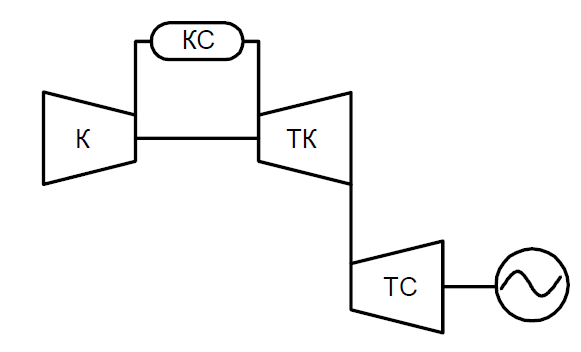
\includegraphics[scale=0.4]{cycle_2n_scheme}
    \caption{Схема двухвальной безрегенеративной установки (К – компрессора, КС – камера сгорания, ТК – турбина компрессора, ТС – силовая турбина)}
    \label{img:cycle_2n_scheme}
\end{figure}

Параметры, характерные для двухавальной безрегенеративной установки, представлены в табл. ~\ref{tab:cycle-2n-parameters}.

\begin{longtable}{|p{7cm}|c|c|c|}
	\caption{Параметры двухвальной безрегенеративной схемы} 
	\label{tab:cycle-2n-parameters}
	\endfirsthead
	\caption*{\tabcapalign Продолжение таблицы~\thetable}\\[-0.45\onelineskip]
	\hline
	\textbf{Величина} & \textbf{Обозначение} & \textbf{Размерность} & \textbf{Значение} \\ \hline
	\endhead
	\hline
	\textbf{Величина} & \textbf{Обозначение} & \textbf{Размерность} & \textbf{Значение} \\ \hline
	Адиабатический КПД компрессора & $\eta_к^*$ & - & 0,82 \\ \hline
	КПД тубины компрессора & $\eta_{тк}^*$ & - & 0,90 \\ \hline
	КПД силовой турбины & $\eta_{тс}^*$ & - & 0,92 \\ \hline
	Номинальная частота вращения вала высокого давления & $n_{0 \ вд} $ об/мин & $12 \cdot 10^3$ \\ \hline
\end{longtable}

Параметры цикла двухвальной безрегенеративной установки на номинальном режиме представлены на рис. ~\ref{img:cycle_2n_opt}.

\begin{figure}[H]
    \centering
    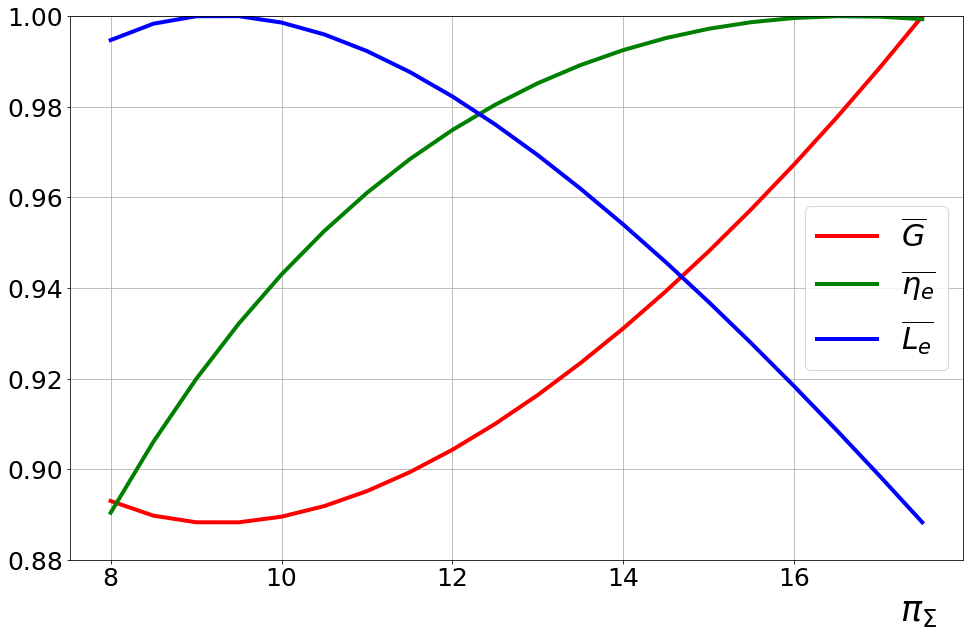
\includegraphics[scale=0.4]{cycle_2n_opt}
    \caption{Параметры цикла двухвальной безрегенеративной установки на номинальном режиме,
	$\overline{G}$ - относительный расход, $\overline{\eta_e}$ - относительный КПД, $\overline{L_e}$ - относительная удельная работа}
    \label{img:cycle_2n_opt}
\end{figure}

В точке, соответствующей максимальному КПД установка имеет параметры, указанные в табл. ~\ref{tab:cycle_2n_max_eta}.

\clearpage
\begin{longtable}{|c|c|c|c|}
	\caption{Параметры двухвальной безрегенеративной установки в точке, соответствующей максимальному КПД}
	\label{tab:cycle_2n_max_eta}
	\hline
	\textbf{$\pi_к$} & \textbf{$L_e, \ МДж/кг$} & \textbf{$\eta_e$} & \textbf{$G_в, \ кг/с$} \\ \hline
	16,5 & 0,270 & 0,325 & 59,2 \\ \hline
\end{longtable}


В точке, соответствующей максимальной удельной работе установка имеет параметры, указанные в табл. ~\ref{tab:cycle_2n_max_labour}.
\begin{longtable}{|c|c|c|c|}
	\caption{Параметры двухвальной безрегенеративной установки в точке, соответствующей максимальной удельной работе} 
	\label{tab:cycle_2n_max_labour}
	\hline
	\textbf{$\pi_к$} & \textbf{$L_e, \ МДж/кг$} & \textbf{$\eta_e$} & \textbf{$G_в, \ кг/с$} \\ \hline
	9,5 & 0,297 & 0,303 & 53,8 \\ \hline
\end{longtable}

В качестве расчетной выбирается точка, соответствующая максимальному КПД.

Параметры двухвальной безрегенеративной схемы представлены на рис. ~\ref{img:cycle_2n_part}.

\begin{figure}[H]
    \centering
    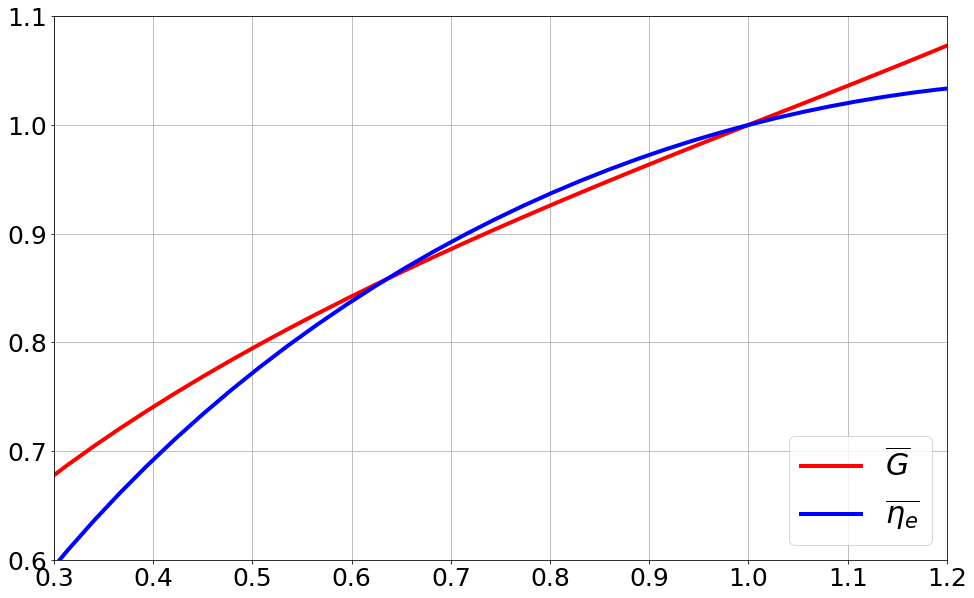
\includegraphics[scale=0.4]{cycle_2n_part}
    \caption{Параметры цикла двухвальной безрегенеративной установки на режимах частичной мощности,
	$\overline{G}$ - относительный расход, $\overline{\eta}$ - относительный КПД, $\overline{N_e}$ - относительная мощность}
    \label{img:cycle_2n_part}
\end{figure}

Двухвальная регенеративная схема преставлена на рис. ~\ref{img:cycle_2nr_scheme}.

\begin{figure}[H]
    \centering
    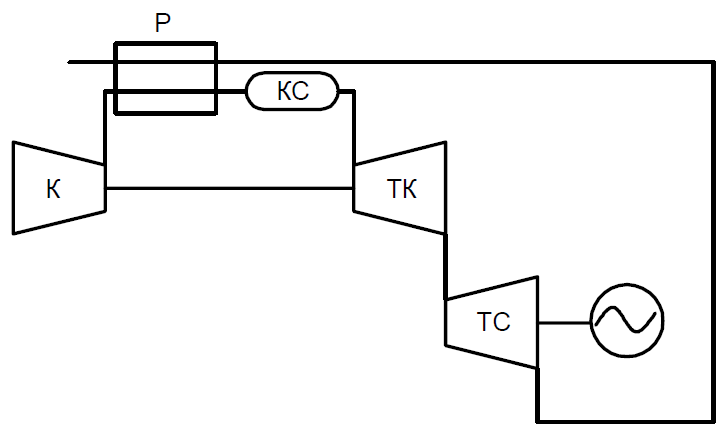
\includegraphics[scale=0.4]{cycle_2nr_scheme}
    \caption{Схема двухвальной регенеративной установки (К – компрессора, КС – камера сгорания, ТК – турбина компрессора, ТС – силовая турбина, Р - регенератор)}
    \label{img:cycle_2nr_scheme}
\end{figure}

Параметры регенеративной двухвальной установки идентичны параметрам установки без регенератора (табл. ~\ref{img:cycle_2n_opt}). Коэффициент регенерации на номинальном режиме $\sigma_р = 0,8$.

Параметры цикла двухвальной безрегенеративной установки на номинальном режиме представлены на рис. ~\ref{img:cycle_2nr_opt}.

\begin{figure}[H]
    \centering
    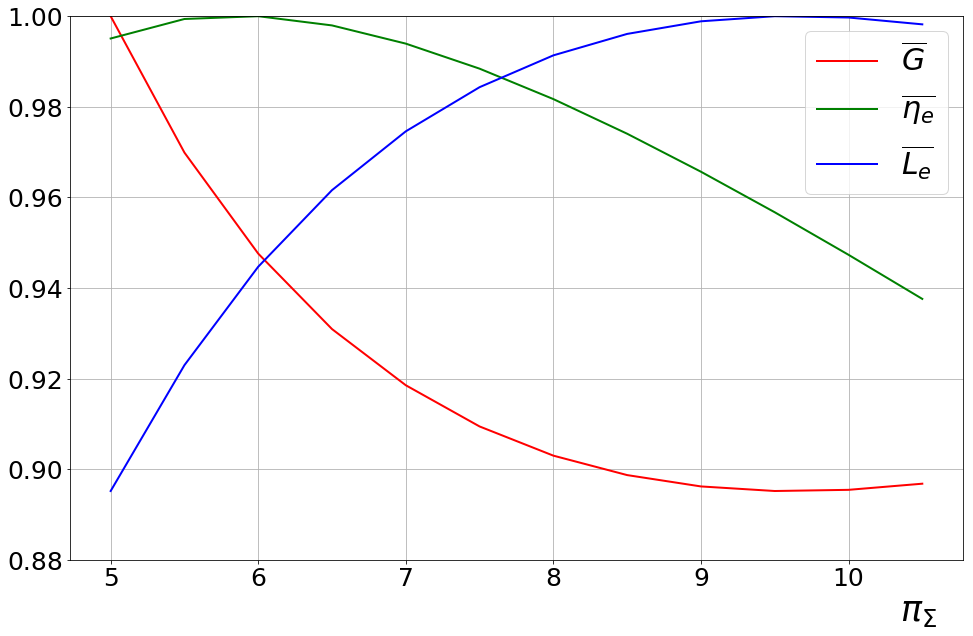
\includegraphics[scale=0.4]{cycle_2nr_opt}
    \caption{Параметры цикла двухвальной регенеративной установки на номинальном режиме,
	$\overline{G}$ - относительный расход, $\overline{\eta_e}$ - относительный КПД, $\overline{L_e}$ - относительная удельная работа}
    \label{img:cycle_2nr_opt}
\end{figure}

В точке, соответствующей максимальному КПД установка имеет параметры, указанные в табл. ~\ref{tab:cycle_2nr_max_eta}.

\begin{longtable}{|c|c|c|c|}
	\caption{Параметры двухвальной регенеративной установки в точке, соответствующей максимальному КПД} 
	\label{tab:cycle_2nr_max_eta}
	\hline
	\textbf{$\pi_к$} & \textbf{$L_e, \ МДж/кг$} & \textbf{$\eta_e$} & \textbf{$G_в, \ кг/с$} \\ \hline
	6,0 & 0,281 & 0,419 & 57,0 \\ \hline
\end{longtable}


В точке, соответствующей максимальной удельной работе установка имеет параметры, указанные в табл. ~\ref{tab:cycle_2n_max_labour}.
\begin{longtable}{|c|c|c|c|}
	\caption{Параметры двухвальной регенеративной установки в точке, соответствующей максимальной удельной работе} 
	\label{tab:cycle_2nr_max_labour}
	\hline
	\textbf{$\pi_к$} & \textbf{$L_e, \ МДж/кг$} & \textbf{$\eta_e$} & \textbf{$G_в, \ кг/с$} \\ \hline
	9,5 & 0,297 & 0,401 & 53,8 \\ \hline
\end{longtable}

В качестве расчетной выбирается точка, соответствующая максимальному КПД.

Параметры двухвальной регенеративной схемы представлены на рис. ~\ref{img:cycle_2nr_part}.

\begin{figure}[H]
    \centering
    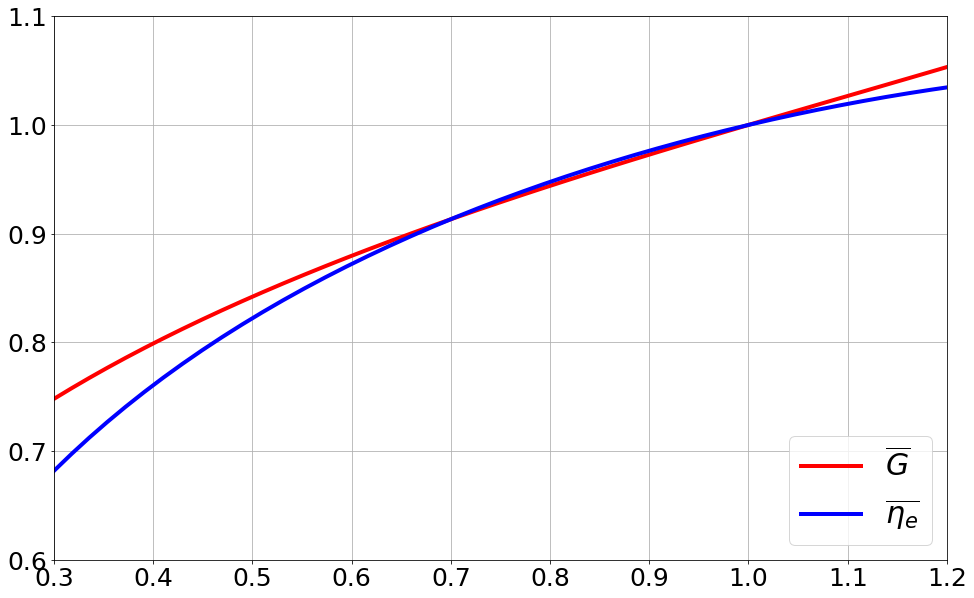
\includegraphics[scale=0.4]{cycle_2nr_part}
    \caption{Параметры цикла двухвальной регенеративной установки на режимах частичной мощности,
	$\overline{G}$ - относительный расход, $\overline{\eta}$ - относительный КПД, $\overline{N_e}$ - относительная мощность}
    \label{img:cycle_2nr_part}
\end{figure}

Трехвальная схема преставлена на рис. ~\ref{img:cycle_3n_scheme}.

\begin{figure}[H]
    \centering
    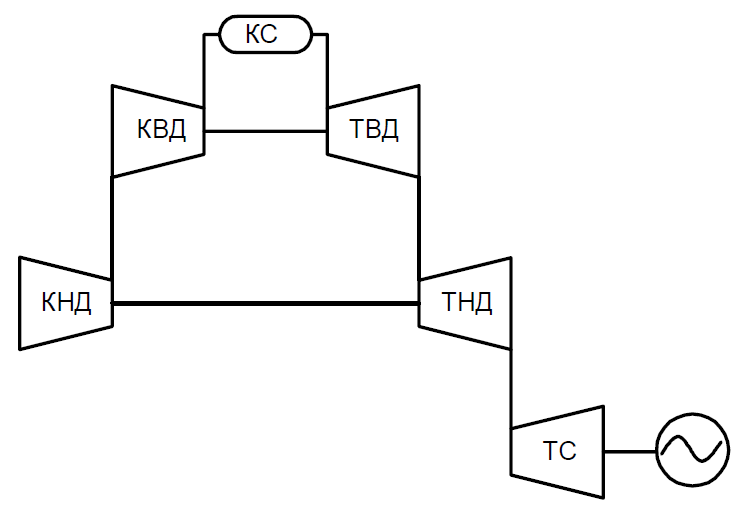
\includegraphics[scale=0.4]{cycle_3n_scheme}
    \caption{Схема трехвальной установки (КНД – компрессор низкого давления, КВД – компрессор высокого давления, КС – камера сгорания, ТВД – турбина высокого давленя, ТНД – турбина низкого давления, ТС – силовая тубина)}
    \label{img:cycle_3n_scheme}
\end{figure}

Параметры, характерные для трехвальной установки, представлены в табл. ~\ref{tab:cycle-3n-parameters}.

\begin{longtable}{|p{7cm}|c|c|c|}
	\caption{Параметры трехвальной схемы} 
	\label{tab:cycle-3n-parameters}
	\endfirsthead
	\caption*{\tabcapalign Продолжение таблицы~\thetable}\\[-0.45\onelineskip]
	\hline
	\textbf{Величина} & \textbf{Обозначение} & \textbf{Размерность} & \textbf{Значение} \\ \hline
	\endhead
	\hline
	\textbf{Величина} & \textbf{Обозначение} & \textbf{Размерность} & \textbf{Значение} \\ \hline
	Адиабатический КПД компрессора низкого давления & $\eta_{кнд}^*$ & - & 0,84 \\ \hline
	Адиабатический КПД компрессора высокого давления & $\eta_{квд}^*$ & - & 0,86 \\ \hline
	КПД турбины низкого давления & $\eta_{тнд}^*$ & - & 0,90 \\ \hline
	КПД турбины высокого давления & $\eta_{твд}^*$ & - & 0,88 \\ \hline
	КПД силовой турбины & $\eta_{тс}^*$ & - & 0,92 \\ \hline
	Номинальная частота вращения вала высокого давления & $n_{0вд}$ & об/мин & 12000 \\ \hline
	Номинальная частота вращения вала низкого давления & $n_{0нд}$ & об/мин & 9500 \\ \hline
\end{longtable}

Параметры цикла трехвальной установки на номинальном режиме представлены на рис. ~\ref{img:cycle_3n_opt}.

\begin{figure}[H]
    \centering
    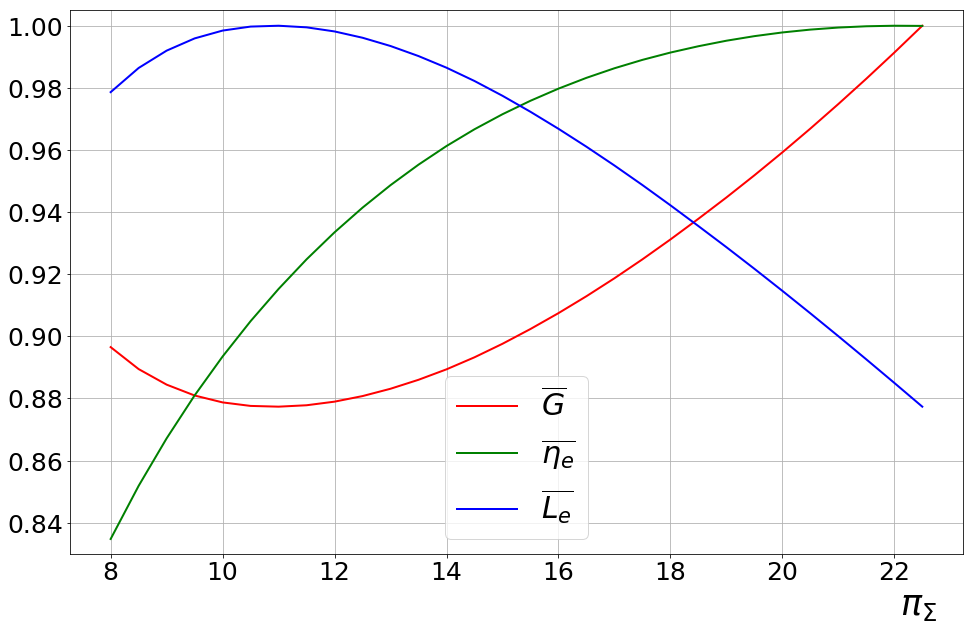
\includegraphics[scale=0.4]{cycle_3n_opt}
    \caption{Параметры цикла трехвальной безрегенеративной установки на номинальном режиме,
	$\overline{G}$ - относительный расход, $\overline{\eta_e}$ - относительный КПД, $\overline{L_e}$ - относительная удельная работа}
    \label{img:cycle_3n_opt}
\end{figure}

В точке, соответствующей максимальному КПД установка имеет параметры, указанные в табл. ~\ref{tab:cycle_3n_max_eta}.

\begin{longtable}{|c|c|c|c|}
	\caption{Параметры трехвальной установки в точке, соответствующей максимальному КПД} 
	\label{tab:cycle_3n_max_eta}
	\hline
	\textbf{$\pi_к$} & \textbf{$L_e, \ МДж/кг$} & \textbf{$\eta_e$} & \textbf{$G_в, \ кг/с$} \\ \hline
	22,0 & 0,279 & 0,392 & 57,4 \\ \hline
\end{longtable}


В точке, соответствующей максимальной удельной работе установка имеет параметры, указанные в табл. ~\ref{tab:cycle_3n_max_labour}.
\begin{longtable}{|c|c|c|c|}
	\caption{Параметры трехвальной установки в точке, соответствующей максимальной удельной работе} 
	\label{tab:cycle_3n_max_labour}
	\hline
	\textbf{$\pi_к$} & \textbf{$L_e, \ МДж/кг$} & \textbf{$\eta_e$} & \textbf{$G_в, \ кг/с$} \\ \hline
	11,0 & 0,315 & 0,321 & 50,8 \\ \hline
\end{longtable}

В качестве расчетной выбирается точка, соответствующая максимальному КПД.

Параметры трехвальной безрегенеративной схемы представлены на рис. ~\ref{img:cycle_3n_part}.

\begin{figure}[H]
    \centering
    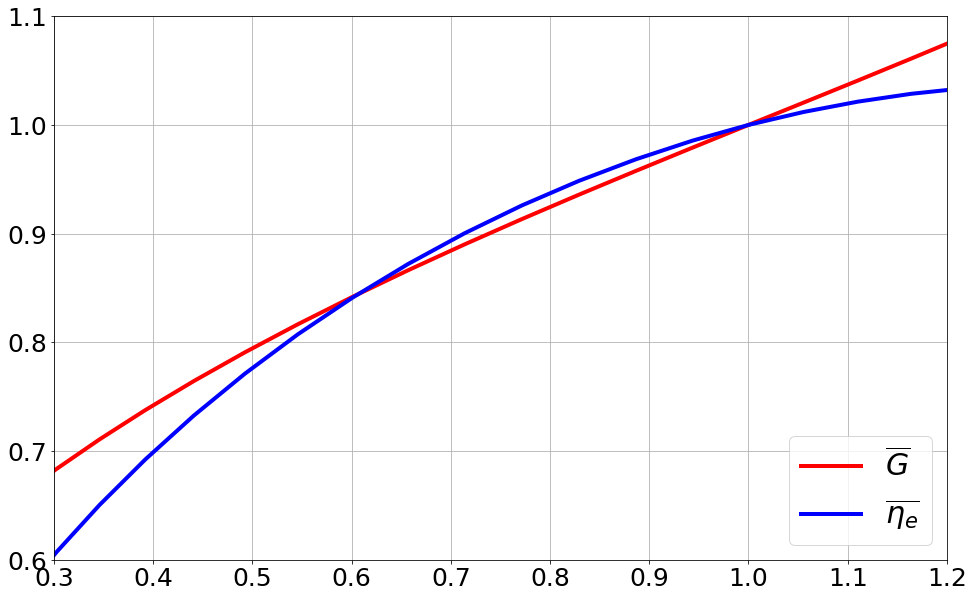
\includegraphics[scale=0.4]{cycle_3n_part}
    \caption{Параметры цикла трехвальной установки на режимах частичной мощности,
	$\overline{G}$ - относительный расход, $\overline{\eta}$ - относительный КПД, $\overline{N_e}$ - относительная мощность}
    \label{img:cycle_3n_part}
\end{figure}

\subsubsection{Анализ полученных данных}
Сравним КПД установок на режимах частичной мощности. Для этого построим зависимости на одном графике зависимости КПД от мощности установки (рис. ~\ref{img:cycle_eta_comparison}). Для удобства отнесем все значения к максимальному КПД из всех установок (номинальному КПД двухвальной регенеративной схемы).

\begin{figure}[H]
    \centering
    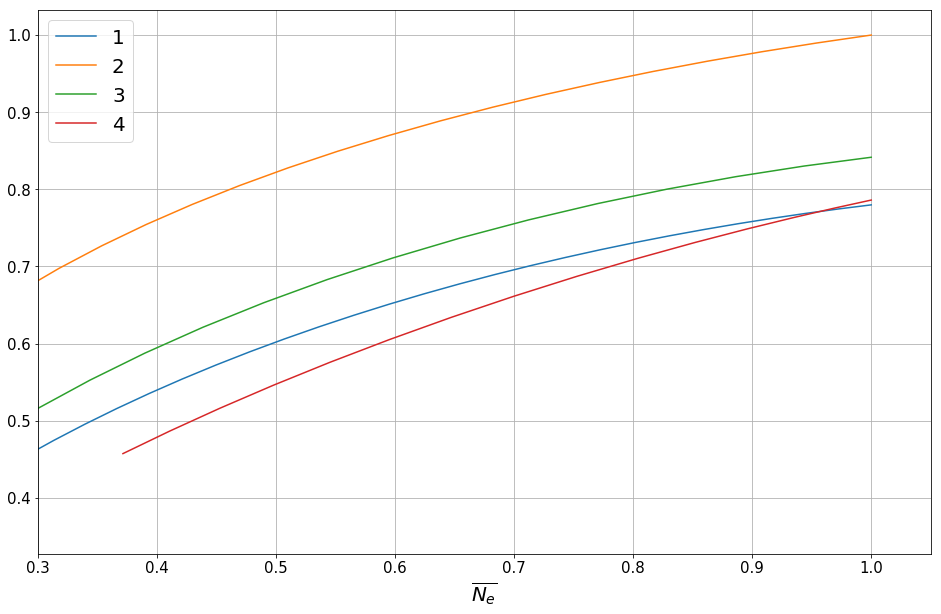
\includegraphics[scale=0.4]{cycle_eta_comparison}
    \caption{Сравнение абсолютных КПД установок (1 – двухвальная безрегенеративная схема, 2 – двухвальная регенеративная схема, 3 – трехвальная схема)}
    \label{img:cycle_eta_comparison}
\end{figure}

Из полученного графика видно, что на всех режимах наиболее эффективным с точки зрения использования топлива является регенеративная схема. Также достоинством данной схемы является снижение удельной работы при снижении мощности установки. Благодаря этому расход в регенеративной схеме по мере уменьшения мощности падает медленнее, чем в безрегенеративной. Однако применение данной схемы приводит к существенному утяжелению установки и увеличению ее инертности, что крайне нежелательно в случае привода ГПА. 

Переход от двухвальной к трехвальной схеме приводит к увеличению КПД установки, за счет увеличения КПД компрессоров и турбин, которые работают при меньшей нагрузке, чем в случае двухвальной схемы. Однако область более высокого КПД сдвигается вправо по суммарной степени повышения давления в установке. В связи с этим предполагаемый рост КПД может быть нивелирован увеличением потерь в радиальном зазоре лопаток КВД и ТВД.

Тем не менее, разработка приводов ГПА мощностью 16 МВт по данной схеме вполне оправдана, так как в этом случае размеры лопаток ТВД и КВД оказываются не меньше нескольких десятков миллиметров.


\subsubsection{Заключение}

В данной исследовании был проведен сравнительный анализ трех схем привода ГПА на 16 МВт: двухвальная безрегенеративная схема, двухвальная регенеративная схема, трехвальная схема. Были рассмотрены термодинамические параметры этих схем как на номинальном режиме, так и на режимах частичной мощности.

Использование регенеративной двухвальной схемы позволило сильно увеличить КПД установки по отношению к безрегенеративному варианту (с 0,325 до 0,419) при уменьшении степени сжатия (с 16,5 до 9,5), что положительно сказывается на КПД лопаточных машин высокого давления. Однако применение регенеративной схемы связано с серьезным увеличением капитальных затрат на производство установки. В связи с этим использование данной схемы в качестве привода ГПА кажется нецелесообразным.
 
 Было показано, что переход к трехвальной схеме позволяет повысить КПД установки (c 0,325 до 0,351) при слабом снижении расхода воздуха (c 59,2 до 57,4 кг/с).
